% Evaluation
\section{Evaluation}
\label{Evaluation}


We implemented Alano in C++ and evaluated the algorithms in a cluster of 9 servers,
each equipped with an Intel Xeon 2.6GHz CPU with 24 hyper-threading cores, 64GB memory and 1T SSD.

We simulated a network that follows uniform distribution and Gaussian distribution respectively.
For uniform distribution, we suppose $500$ nodes are distributed in an area of $100m \times 100m$ and each node's communication range is $\Delta = 10m$. For Gaussian distribution, we suppose $1000$ nodes are distributed in the same area, but each node's communication range is $\Delta = 5m$. We set the Gaussian distribution as $N(50,15^2)$ in our evaluation.
We set time slot length to be $20ms$ and duty cycle of a node to be $0.1$ for symmetric nodes; for asymmetric nodes, we set their duty cycle randomly from $0.05$ to $0.15$ with step $0.02$.

These settings make the network more complicated and realistic than that in
\cite{wang2015blinddate, qiu2016talk, sun2014hello, bakht2012searchlight,
chen2015heterogeneous, kandhalu2010u, you2011aloha,
mcglynn2001birthday, song2014probabilistic, vasudevan2009neighbor}.



We evaluated discovery latency of Alano, Aloha-like~\cite{you2011aloha}, Hello~\cite{sun2014hello}, Hedis~\cite{chen2015heterogeneous}, and Searchlight~\cite{bakht2012searchlight} in the generated partially-connected networks. Besides, we evaluated G-Nihao(we choose the best parameters, $m=n$, $\alpha=0.054$)~\cite{qiu2016talk}, but $500$ symmetric nodes in uniform distribution can only discover $2\%$ neighbors, which is worse than other $3$ deterministic algorithms we choose. Thus, we didn't show its result in our figures.
Hedis only has two states $\{ON, OFF\}$ (representing the radio is on or off). To make the comparison more fair, we assume that when a node is in $\{ON\}$ state, it transmits or listens with equal probability $0.5$. Hello and Searchlight has a beacon transmission of $0.54ms$ at the beginning and end of each slot, and a beacon makes up about $1/40$ of a slot, so we divide each $\{ON\}$ slot into $40$ mini-slots, and the node transmits at the first and last mini-slot, and listens in other mini-slots.
In the following parts, we show that Alano has lower latency, higher discovery rate, better scalability, and better robustness.

\subsection{Speed: Discovery Latency}

\begin{figure}[!h]
\centering
\subfigure[Uniform Distribution]{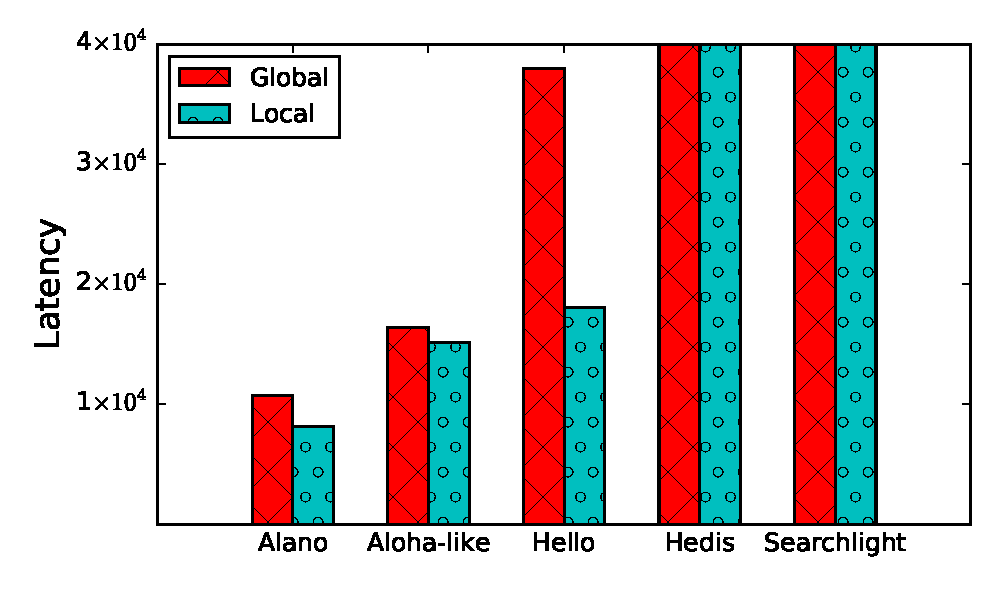
\includegraphics[width=1.65in]{Figure/latency_uniform}}
\hspace{0.01in}
\subfigure[Gaussian Distribution]{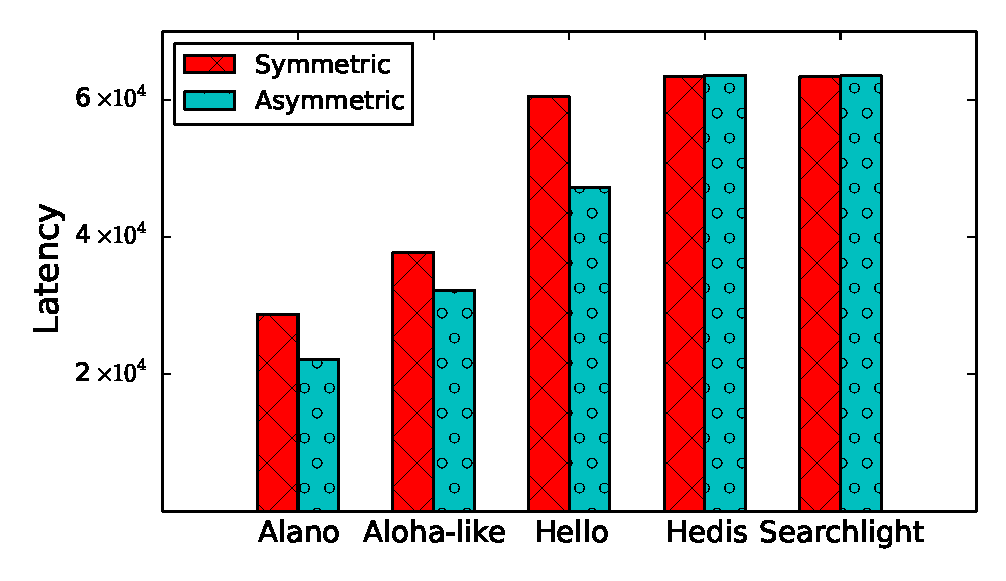
\includegraphics[width=1.65in]{Figure/latency_normal}}
\caption{Alano achieves lower latency.}
\label{fig_latency}
\end{figure}

When nodes follow uniform distribution, we show the discovery latency comparison for both symmetric nodes and asymmetric nodes in Fig. \ref{fig_latency}(a).
From the figure, Alano achieves $54.64\%$ to $1.95$ times lower discovery latency for symmetric nodes, and $85.25\%$ to $2.91$ times lower discovery latency for asymmetric nodes.
When nodes follow Gaussian distribution, as depicted in Fig. \ref{fig_latency}(b), 
Alano achieves $31.35\%$ to $1.21$ times lower discovery latency for symmetric nodes, and $45.94\%$ to $1.88$ times lower discovery latency for asymmetric nodes.
The deterministic algorithms, Hello, Hedis and Searchlight, have high latency because these protocols only considered the bounded latency between two nodes. When the network becomes denser and a node has many neighbors, they cannot discover rapidly due to communication collisions.


\subsection{Quality: Discovery Rate}

% \begin{figure}[!h]

% \subfigure[Uniform Distribution with Global Duty Cycle]{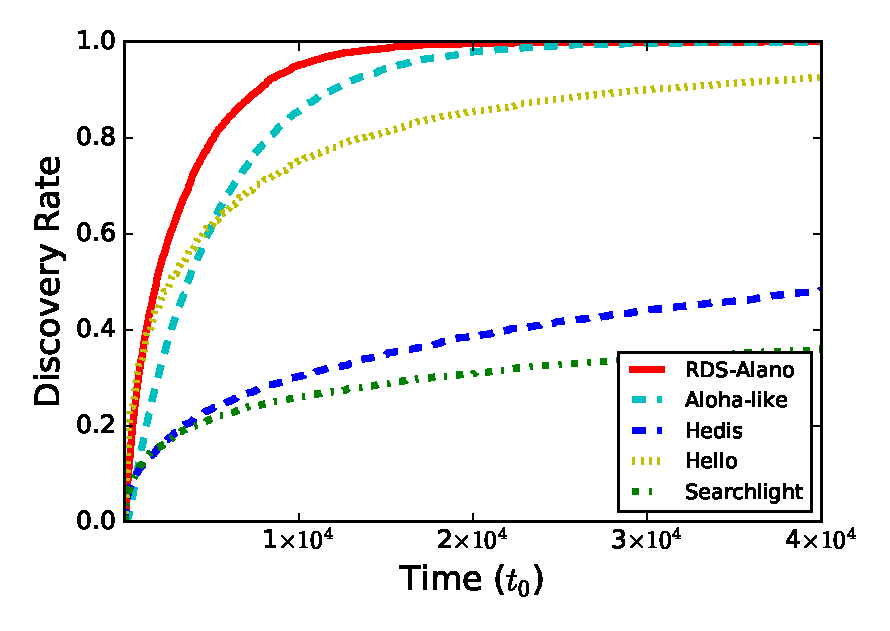
\includegraphics[width=1.65in]{Figure/rate_uniform}}
% \hspace{0.01in}
% \subfigure[Normal Distribution with Global Duty Cycle]{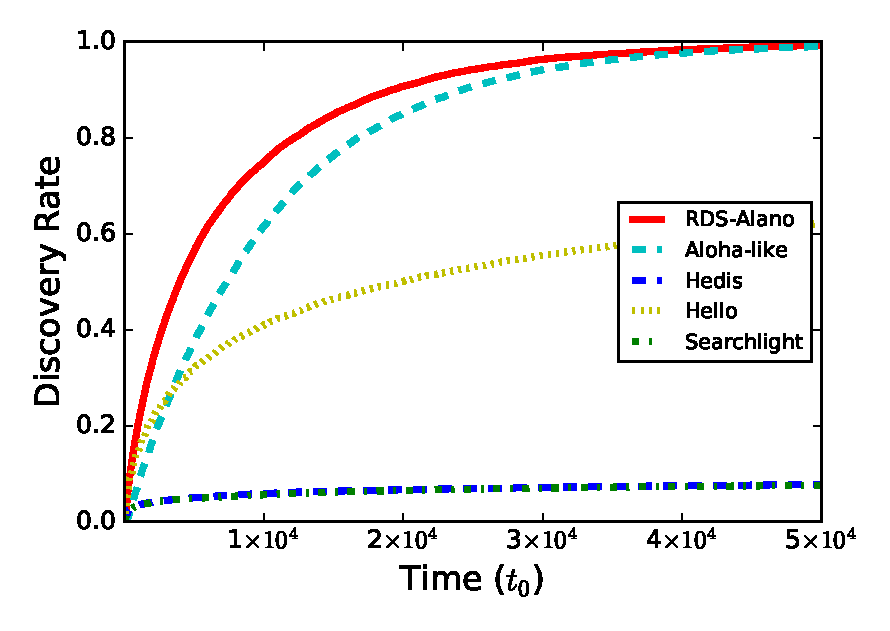
\includegraphics[width=1.65in]{Figure/rate_normal}}
% \hspace{0.01in}
% \subfigure[Uniform Distribution with Local Duty Cycle]{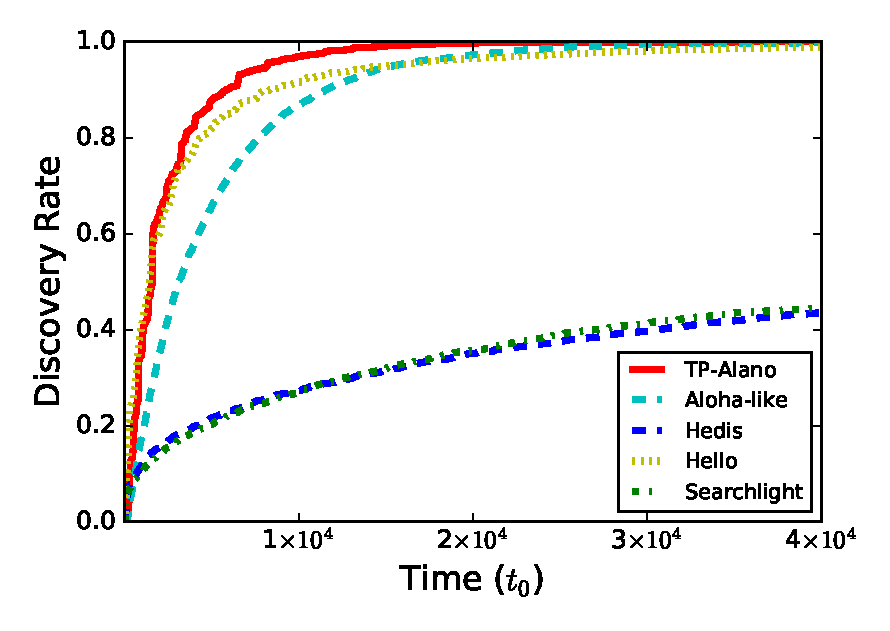
\includegraphics[width=1.65in]{Figure/rate_local_uniform}}
% \hspace{0.01in}
% \subfigure[Normal Distribution with Local Duty Cycle]{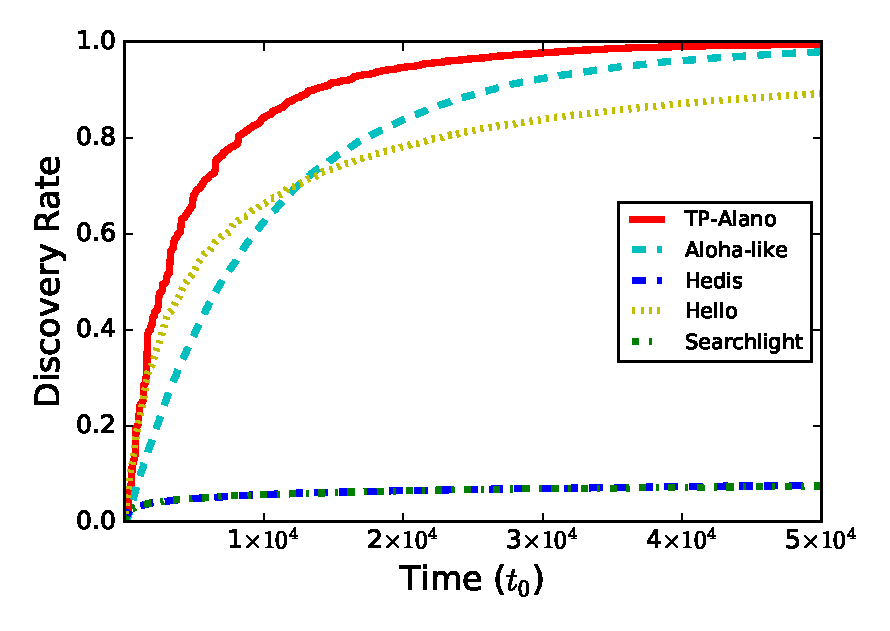
\includegraphics[width=1.65in]{Figure/rate_local_normal}}
% \caption{Alano achieves higher discovery rate.}
% \label{fig_timerate}
% \end{figure}


% Fig. \ref{fig_timerate} shows Alano with either global or local duty cycle, has higher discovery rate during the whole course of neighbor discovery in both uniform and normal distribution. The deterministic algorithms Hello, Hedis and Searchlight cannot discover all channels, because of the occurence of collisions. Aloha-like discovers more slowly than Alano when it has discovered a certain number of channels, such as $80\%$ channels in Uniform Distribution with Global Duty Cycle, because it is difficult for pure probabilistic algorithm to deal with the small amount of   undiscovered neighbors.

\begin{figure}[!h]

\subfigure[Symmetric Nodes in Uniform Distribution]{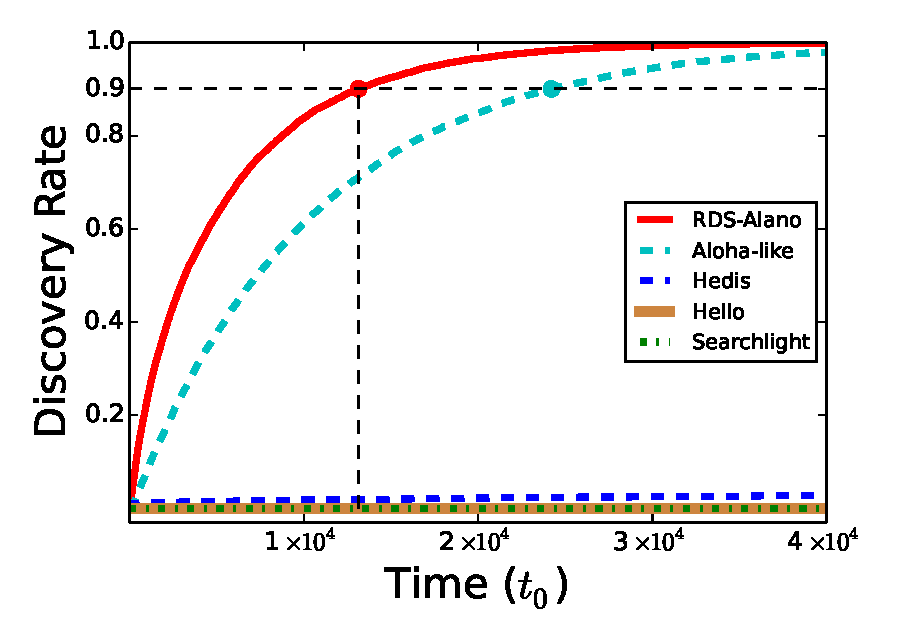
\includegraphics[width=1.65in]{Figure/rate_uniform1}}
\hspace{0.01in}
\subfigure[Symmetric Nodes in Gaussian Distribution]{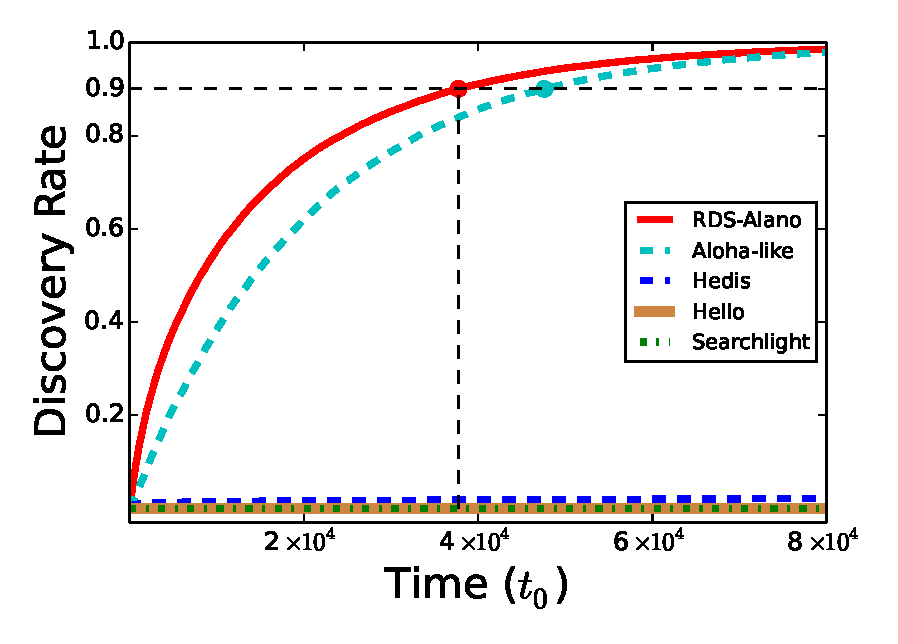
\includegraphics[width=1.65in]{Figure/rate_normal1}}
\hspace{0.01in}
\subfigure[Asymmetric Nodes in Uniform Distribution]{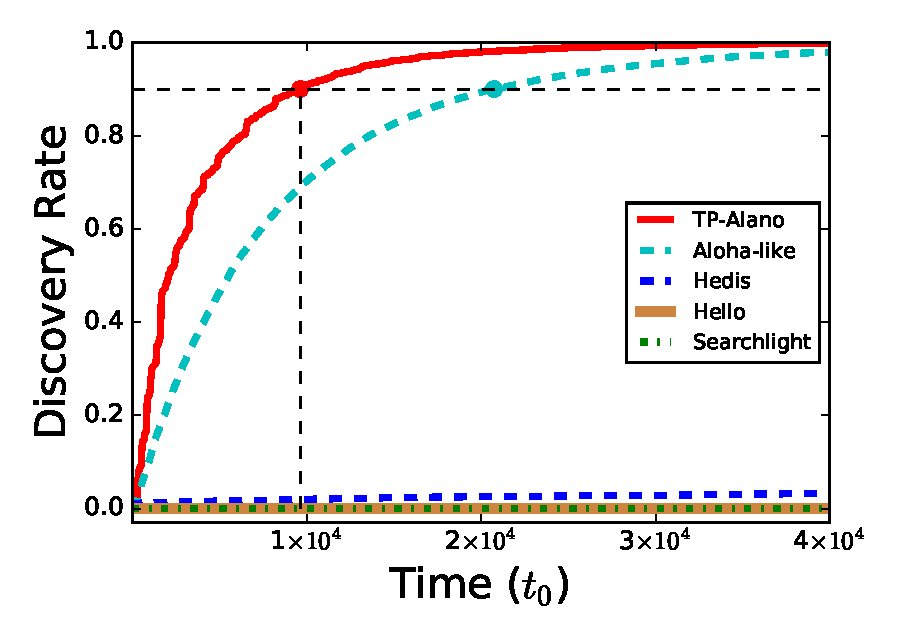
\includegraphics[width=1.65in]{Figure/rate_local_uniform1}}
\hspace{0.01in}
\subfigure[Asymmetric Nodes in Gaussian Distribution]{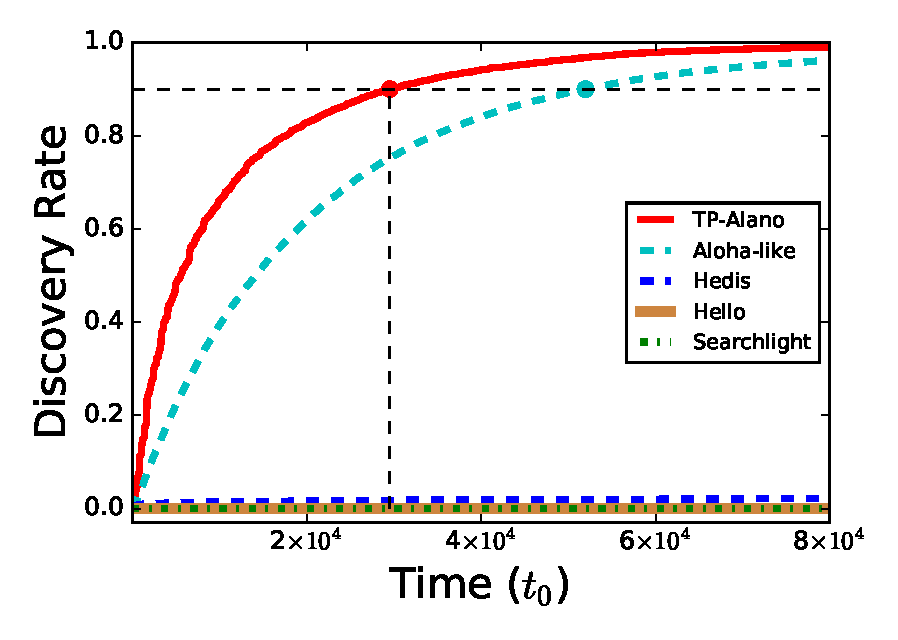
\includegraphics[width=1.65in]{Figure/rate_local_normal1}}
\caption{Alano achieves higher discovery rate in larger networks.}
\label{fig_timerate_large}
\end{figure}


% (??define discovery rate)
% (??some places you use normal distribution, but some places you use Gaussian distribution, correct them)
We use discovery rate to evaluate Alano's quality.
Discovery rate of a node $u_i$ is defined as the percentage of discovered neighbors over $u_i$'s all neighbors.
In Fig. \ref{fig_timerate_large}, we increase the number of nodes from $500$ to $1000$ for the uniform distribution, and increase the number of nodes from $1000$ to $2000$ for the Gaussian distribution, the results show that Alano has higher discovery rate during the whole process for both uniform and Gaussian distributions. The deterministic algorithms, Hello, Hedis and Searchlight, cannot discover all nodes due to the occurrence of collisions.
%Aloha-like discovers more slowly than Alano when it has discovered a certain number of channels, such as $80\%$ channels in Uniform Distribution with Global Duty Cycle, because it is difficult for pure probabilistic algorithm to deal with the small amount of   undiscovered neighbors.





\subsection{Scalability: Duty Cycle and Network Density}

We evaluated Alano's scalability regarding duty cycle and network density.

\begin{figure}[!h]
\centering
\subfigure[Uniform Distribution]{\includegraphics[width=1.65in]{Figure/dutycycle_uniform}}
\hspace{0.01in}
\subfigure[Gaussian Distribution]{\includegraphics[width=1.65in]{Figure/dutycycle_normal}}
\caption{Alano achieves lower latency in different duty cycle.}
\label{fig_dutycycle}
\end{figure}


\emph{1. Duty Cycle}
%(?? not clear, symmetric nodes or asymmetric nodes)
When symmetric nodes with different duty cycles, Fig. \ref{fig_dutycycle} shows that Alano has lower latency. Compared with Aloha, Alano has from $53.66\%$ to $11.23$ times lower latency. The latency of Alano and Aloha generally decreases as the duty cycle increases, while Hello, Hedis and Searchlight have high latency due to the collision. In Gaussian distribution, Alano has a small twist with duty cycle $0.35$, because when the duty cycle increases, nodes are more likely to transmit and therefore collide.


\emph{2. Network Density}

When the number of nodes increases, the network becomes denser. We choose Aloha-like algorithm for comparison because Hello, Hedis and Searchlight already have higher latency than Aloha-like when there are $500$ nodes in uniform distribution and $1000$ nodes in Gaussian distribution.
As shown in Fig. \ref{fig_node}(a), Alano achieves $4.68$ times to $6.51$ times lower discovery latency than Aloha-like algorithm for uniform distribution, when the number of nodes increases from $1000$ to $9000$.
When the number of nodes increases from $1000$ to $9000$ for Gaussian distribution, Alano achieves $25.23\%$ to $1.03$ times lower discovery latency as shown in Fig. \ref{fig_node}(b).  

\begin{figure}[!h]
\centering
\subfigure[Uniform Distribution]{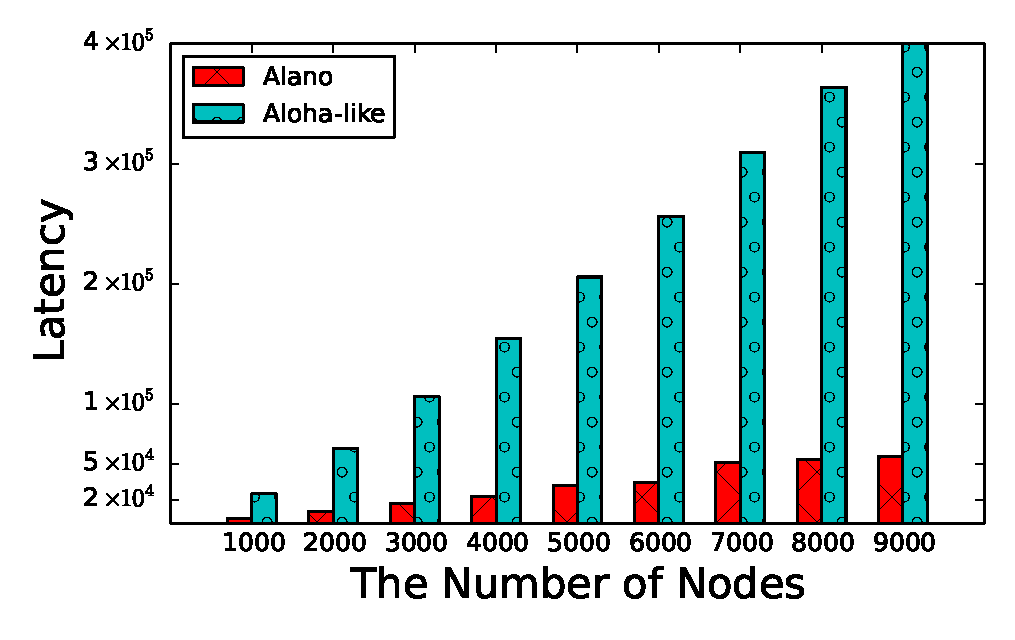
\includegraphics[width=1.65in]{Figure/node_uniform}}
\hspace{0.01in}
\subfigure[Gaussian Distribution]{\includegraphics[width=1.65in]{Figure/node_normal}}
\caption{Alano achieves lower latency with different number of nodes.}
\label{fig_node}
\end{figure}

% \subsection{Robustness}

% \begin{figure}[!h]
% \centering
% \subfigure[Uniform Distribution]{\includegraphics[width=1.65in]{Figure/robustU}}
% \hspace{0.01in}
% \subfigure[Gaussian Distribution]{\includegraphics[width=1.65in]{Figure/robustN}}
% \caption{Alano still reaches low latency when nodes die.}
% \label{fig_robust}
% \end{figure}

% In reality, a node may leave the network now and then (such as the node runs out of energy or the node is offline for other usage). We evaluate the robustness of the neighbor discovery algorithms in Fig. \ref{fig_robust}. When $5\%$ to $30\%$ nodes die (see x-axis of the figure), Alano still reaches low discovery latency for both uniform and Gaussian distributions. %(?? others?)
